	\subsection{Percorrenza di un Treno}
	
	A ciascuna entità Treno, è assegnato un Percorso (\ttt{Route}) di andata e un Percorso di ritorno, ovvero sequenze di Tappe (\ttt{Stage}) successive, ciascuna composta dai seguenti campi:
				\begin{center}
					\begin{verbatim}
    - start_station,
    - start_platform,
    - next_segment,
    - next_station,
    - next_platfom,
    - leave_action,
    - enter_action,
    - node_name
					\end{verbatim}
				\end{center}
dove \ttt{leave\_action} e \ttt{enter\_action} indicano rispettivamente quello che un Treno dovrà compiere alla partenza dalla stazione \ttt{start\_station} e all'arrivo presso la prossima stazione \ttt{next\_station}, a scelta tra \ttt{ENTER}, per entrare ed effettuare discesa e salita passeggeri o \ttt{PASS} per non fermarsi e oltrepassare la Stazione; il campo \ttt{node\_name} invece, indica la regione di destinazione, e viene utilizzato nel caso di transito su stazione di Gateway.

Una volta che un thread del pool della struttura \ttt{Train\_Pool} ottiene un Descrittore, effettua le seguenti  operazioni, per ciascuna Tappa del Percorso corrente (di andata o di ritorno):
				\begin{itemize} 
					\item Partenza dalla Stazione \ttt{start\_station}, Piattaforma \ttt{start\_platfom}.
					\item Accesso al prossimo Segmento \ttt{next\_segment}.
					\item Percorrenza all'interno del Segmento come attesa finita di durata proporzionale alla lunghezza del Segmento e alla velocità massima alla quale il Treno può percorrerlo.
					\item Uscita dal Segmento e richiesta di Accesso alla Stazione successiva (\ttt{next\_station}) presso la Piattaforma indicata da \ttt{next\_platfom}, per eseguire l'azione \ttt{action}.
					\item Se \ttt{action = ENTER} allore effettua discesa e salita dei Viaggiatori in attesa dell'arrivo del Treno.
					\item Se ci sono ancora Tappe da percorrere nel percorso (\ttt{Route}), allora il l'indice della prossima tappa del Descrittore del Treno corrente viene incrementato, e lo stesso Descrittore viene inserito in una delle code di \ttt{Train\_Pool} (in base alla priorità). 
				\end{itemize}

% ############################################################################################################
% ################################################# ACCESSO_SEGMENTO #########################################
% ############################################################################################################
	
		\subsubsection{Accesso ad un Segmento}
		
		L'accesso alla risorsa protetta Segmento è regolato da una interfaccia ben definita, che permette:
			\begin{itemize}
				\item Ingresso.
				\item Uscita.
			\end{itemize}
		Per mantenere l'ordine di accesso, ciascun Segmento è dotato di una Coda FIFO (\ttt{Train\_Queue}) che conterrà i Descrittori dei Treni correntemente in transito. Tale coda avrà una capienza massima per limitare il numero di accessi consecutivi da una singola direzione.
		
		\begin{description}
			
			\item {\ii{Ingresso}} \\
			
			La richiesta di accesso (\ttt{Enter}) al segmento avviene in mutua esclusione tra tutti le entità Treno. In ogni momento quindi solo una entità eseguirà all'interno della risorsa protetta. Una volta ottenuta la risorsa ciascun Treno compie le seguenti operazioni
			 \begin{itemize}
			 	\item Inserimento del Descrittore nella coda \ttt{Train\_Queue};
			 	\item Aggiornamento della velocità di percorrenza del Treno entrato in base a quella dei treni che lo precedono.
			 	\item Nel caso in cui la risorsa risulti vuota (viene consultato il flag booleano che mantiene questa informazione), allora viene modificato il valore del flag in modo tale da indicare lo stato occupato della risorsa, e memorizzata la stazione di provenienza del Treno.
			\end{itemize}
			Una volta terminate queste due operazioni, il Treno rilascia la risorsa e, basandosi sulla lunghezza e sulla velocità da mantenere, simula la percorrenza rendendosi inattivo (non competitivo per l'ottenimento della CPU) per un tempo dato dalla semplice equazione: $ Time = Segment\_Length / Actual\_Speed $.
			
			Nel permettere percorrenza multipla del Segmento, si presentano diverse problematiche: nel caso in cui una volta ottenuta la risorsa protetta Segmento, un Treno richieda l'accesso nella direzione opposta a quella dei Treni che percorrono il Segmento (ovvero abbiamo la situazione in cui il flag booleano \ttt{Free = False}, e la stazione di provenienza memorizzata presso il Segmento è diversa da quella del Treno richiedente) allora questo dovrà attendere fino a che il Segmento non sarà si sarà liberato dai treni in transito. Questa attesa dev'essere tale da evitare starvation del Treno in attesa.
			
			Una primo approccio possibile è quello di prevedere una coda di attesa interna alla risorsa Segmento (\ttt{Waiting\_Queue}), per i Treni provenienti dalla direzione opposta rispetto al senso di marcia corrente: tali Treni dovranno avere priorità maggiore nell'accedere al Segmento appena esso diventa vuoto, rispetto ad altri Treni che sopraggiungono successivamente.
			Questo però, non risulta sufficiente a garantire che i Treni nella coda avranno accesso al Segmento in qualche momento: si consideri la presenza di un percorso circolare composto da $N$ Segmenti, e di $M$ Treni che viaggiano lungo tale percorso in senso orario, in modo tale che in ogni istante ci sia almeno un treno all'interno di ciascun Segmento. Se ora aggiungiamo al sistema un Treno che viaggia in direzione opposta, allora esso, adottando la semantica di accesso descritta non riuscirà mai a percorrere uno dei Segmenti.			
			
			Una possibile soluzione al problema, è mantenere nella coda \ttt{Waiting\_Queue} \ii{tutte} le entità Treno che non possono accedere correntemente, sia perché provenienti dalla direzione opposta, sia perché il numero massimo di accessi da una direzione è stato raggiunto. In questo modo la semantica di accesso viene modificata come segue:
				\begin{itemize}
					\item Se \ttt{Free = True} allora il Treno corrente 
						\begin{itemize}
							\item Modifica il valore di \ttt{Free} a \ttt{False}.
							\item Imposta la Stazione provenienza con la propria.
							\item Incrementa di 1 il contatore di accessi.
						\end{itemize}
					\item Se invece \ttt{Free = False} allora
						\begin{itemize}
							\item Se la stazione di provenienza del Treno corrente è diversa da quella memorizzata nel Segmento, allora inserisci il Treno nella coda \ttt{Waiting\_Queue} e STOP.
							\item Altrimenti 
								\begin{itemize}
									\item Se il contatore di accessi è $ < $ del limite massimo di Treni provenienti da una singola direzione, allora incrementa di 1 il contatore di accessi.
									\item Altrimenti accoda il Treno su \ttt{Waiting\_Queue} e STOP.
								\end{itemize}
						\end{itemize}
					\item Se il Treno ha avuto accesso al Segmento, inserisci il Descrittore del Treno nella coda \ttt{Train\_Queue} e modifica velocità di transito del Treno a seconda della massima velocità possibile.
				\end{itemize}
			  
			\item {\ii{Uscita}} \\ 
			
			L'uscita (\ttt{Leave}) da una Segmento da parte di una entità Treno, ha come prerequisito l'aver avuto accesso al Segmento. \'E quindi possibile assumere che il descrittore del Treno che intende uscire dal Segmento sia presente all'interno della coda \ttt{Train\_Queue}, e che inoltre al momento di tale richiesta abbia già terminato il tempo previsto di attesa che simula la percorrenza.
			
			Il requisito principale richiesto dall'azione di uscita è che essa avvenga in maniera ordinata, in base all'ordine con cui i Treni hanno avuto accesso al Segmento. La soluzione apportata mira a garantire tale ordine di uscita, senza fare alcuna assunzione sull'ordine con il quale i Treni verranno scelti per l'esecuzione dallo scheduler. La semantica adottata è quindi la seguente:
			\begin{itemize}
				 \item Viene controllato per prima cosa se il Treno corrente è effettivamente il prossimo che deve uscire secondo l'ordine di ingresso.
				 \item Se è è il prossimo (vengono confrontati i Descrittori) allora il Treno può abbandonare la risorsa protetta.
				 \item Altrimenti il Descrittore del Treno corrente viene posto in attesa su una coda; tale coda verrà riesaminata ogni volta che un Treno abbandonerà la risorsa protetta (disponendo ad esempio di instruzioni wait e signal, ciascun Treno uscente invocherà una signal sulla coda), e se il Treno in esecuzione non sarà nuovamente il Treno destinato ad uscire, esso verrà riaccodato. 
			\end{itemize}
		\end {description}  
	
	La semantica descritta, garantisce ingresso sequenziale a molteplicità limitata, e uscita ordinata secondo l'ordine di ingresso. Il passo successivo consiste nel garantire l'accesso alla Stazione con lo stesso ordine di uscita per tutti i Treni provenienti dallo stesso Segmento.

% ############################################################################################################
% ####################################### ACCESSO_STAZIONE_REGIONALE #########################################
% ############################################################################################################

		\subsubsection{Accesso ad una Stazione Regionale}\label{subsubsec:regional_station_access}
		
		\begin{figure}[htbp]
			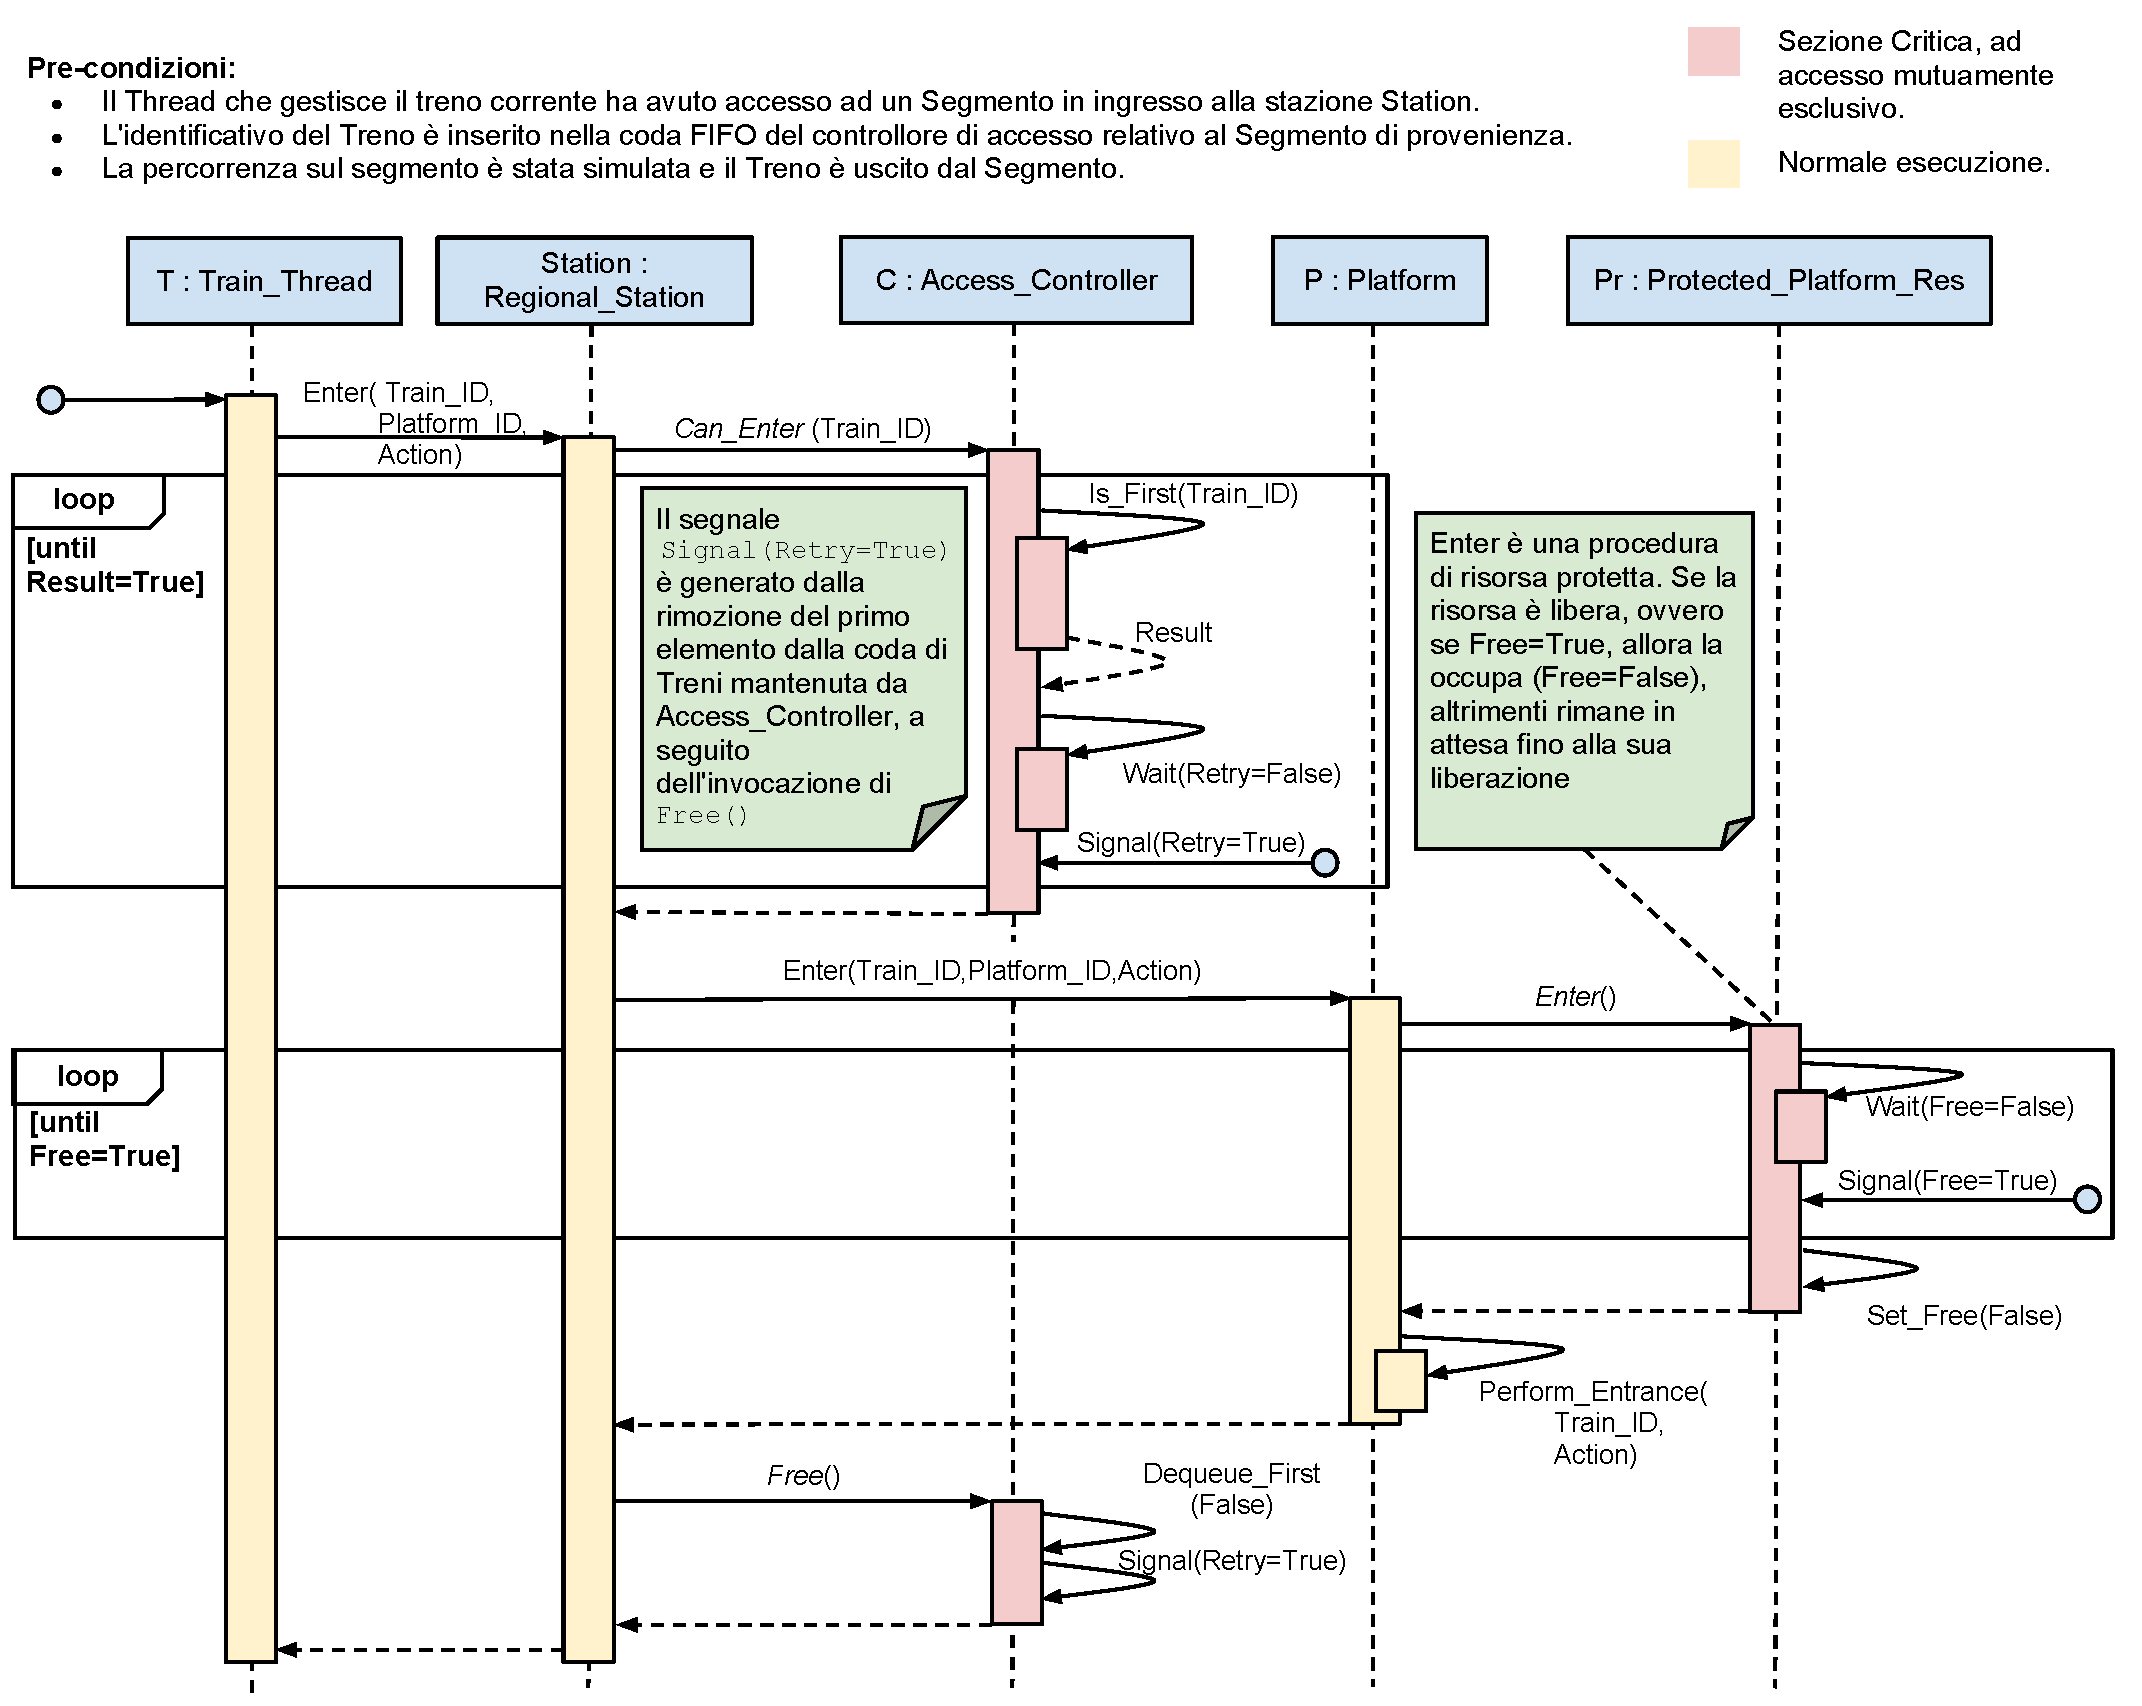
\includegraphics[trim = 40mm 0mm 0mm 0mm,scale=0.5]{imgs/platform_access_Sequence_Diagram.pdf}
			\caption{\footnotesize{Diagramma di Sequenza, operazioni necessarie per l'ingresso ad una Piattaforma.}}
			\label{fig:platform_access}
		\end{figure}
		
		I prerequisiti alla richiesta da parte di un Treno $T$ di accesso ad una Stazione sono:
		
			\begin{itemize}
				\item Il Treno $T$ ha avuto accesso ad un Segmento $S$ che collega la stazione corrente a quella dalla quale proviene. Ciò significa che il suo Descrittore sarà stato inserito nella coda \ttt{Train\_Queue} di $S$.
				\item Il Treno $T$ ha simulato la percorrenza su $S$ 
				\item Il Treno $T$ uscito dal Segmento $S$, quindi è stato rimosso dalla coda \ttt{Train\_Queue} di $S$.
			\end{itemize}
			
		Il diagramma di sequenza in figura \ref{fig:platform_access} mostra le operazioni che portano alla richiesta ordinata di accesso, e all'ingresso presso una Piattaforma.
		\begin{description}
	% ################################################# INGRESSO_ORDINATO #########################################
			\item{\ii{Ingresso Ordinato}}\\
		
		Per tutti i Treni provenienti dallo stesso Segmento, è necessario mantenere un ordine di richiesta di accesso alla Stazione successiva uguale a quello utilizzato per l'uscita dal Segmento. Poiché il sistema non può fare assunzioni sulle scelte dello scheduler che verrà adottato, è necessario introdurre un meccanismo che riesca a mantenere l'ordine di richiesta di accesso anche nel caso in cui, il thread che rappresenta il Treno appena uscito dal Segmento venga prerilasciato e venga eseguito il thread rappresentante il Treno successivo.

		Ho vagliato le seguenti soluzioni possibili:
		\begin{enumerate}
			\item Rappresentazione della Stazione come entità passiva ad accesso mutuamente esclusivo. Essa mantiene al suo interno una coda per Segmento, del tutto simile alla coda \ttt{Train\_Queue} interna ai Segmenti, e popolata parallelamente a \ttt{Train\_Queue}. In questo modo è semplice garantire (con un meccanismo simile a quello utilizzato per l'uscita da un Segmento) un accesso ordinato. Questa soluzione ha però uno svantaggio evidente: la richiesta di accesso avviene in mutua esclusione anche tra i Treni provenienti da Segmenti diversi, e che quindi si ritroveranno a dover superare un punto di sincronizzazione inutile, se diretti a Piattaforme diverse della Stazione.
			
			\item Una seconda possibilità prevede la presenza, all'interno di ciascuna Stazione, di una risorsa ad accesso mututamente esclusivo per ciascun Segmento entrante, la quale si occuperà di garantire l'ordine di accesso (tale ordine sarà dato da una coda interna aggiornata in modo analogo alla soluzione precedentemente illustrata). Una volta che il Treno ha guadagnato il permesso di accedere in mutua esclusione alla risorsa protetta di controllo, esso avrà il permesso di accedere alla Piattaforma corretta, in modo concorrente con i Treni provenienti da altri Segmenti entranti. La coda con politica di ordinamento FIFO che indicherà l'ordine di accesso, sarà aggiornata dal Segmento mediante un'invocazione ad una procedura di interfaccia della Stazione (ad esempio \ttt{Add\_Train}).
			In questo modo la Stazione diventerà solo un'interfaccia utilizzabile per l'accesso alle piattaforme, e inoltre i vincoli di ordinamento e accesso concorrente alle Piattaforme da Treni provenienti da Segmenti diversi saranno garantiti.
			
			Lo svantaggio di utilizzare questa soluzione risiede nella creazione delle entità protette, una per ciascun Segmento entrante, che regolano l'accesso ordinato, e quindi spostano parte della conoscenza della topologia della rete ferroviaria anche sulle Stazioni, rendendone più complessa la configurazione iniziale.
			
			\item La terza soluzione esaminata, che è quella effettivamente utilizzata nel progetto, è simile alla soluzione precedente, ma a differenza di essa opera una popolazione dinamica della struttura dati che andrà a contenere le risorse protette (\ttt{Access\_Controller}) che garantiscono l'ordinamento. Ciascun Treno nell'accedere alla Stazione, includerà anche un'identificativo univoco del Segmento di provenienza, e se per esso non esisterà una controllore degli accessi, allora esso verrà creato. Questa variante ha il vantaggio per il quale le stazioni non devono necessariamente essere a conoscenza della topologia del sistema ferroviario; inoltre l'allocazione di controllori sarà limitata al massimo al numero di Segmenti in ingresso.
		\end{enumerate} 
		
		Il controllore di accessi (\ttt{Access\_Controller}) ha quindi il compito di fornire da semaforo internamente alla Stazione, in modo tale ogni volta da lasciar passare solamente il Treno (il thread che lo esegue) che effettivamente è primo nella coda. Siano \ttt{Enter} e \ttt{Leave} rispettivamente le due procedure protette del semaforo, allora l'accesso alla Piattaforma verrà regolato nel seguente modo:
			\begin{itemize}
				\item Il Treno $T$ usa \ttt{Enter} per poter accedere alla prossima Piattaforma.
				\item Se $T$ è effettivamente il primo della Coda allora 
					\begin{itemize}
						\item prosegue all'\ii{accesso alla Piattaforma};
						\item libera l'\ttt{Access\_Controller} con \ttt{Free}. 
					\end {itemize}
				\item Altrimenti viene messo in attesa del proprio turno su una apposita coda (anch'essa FIFO). I Treni in attesa su questa coda verranno risvegliati ogni volta che un Treno effettuerà un accesso e una successiva chiamata a \ttt{Free}.
			\end{itemize}
		
	% ############################################## INGRESSO_PIATTAFORMA #########################################
		\item{\ii{Ingresso in una Piattaforma}}\\
		
		Dopo aver superato la risorsa di controllo \ttt{Access\_Controller}, ciascun Treno è libero di richiedere l'accesso alla Piattaforma successiva prevista dal percorso, interna a ciascuna Stazione, poiché sicuramente sarà l'unico ad eseguire a questo punto. La semantica di accodamento su di una generica Piattaforma $P$ (supponiamo disponibile mediante procedura eseguita in mutua esclusione) è la seguente:
		\begin{itemize}
			\item Se $P$ è libera, ovvero il flag booleano \ttt{Free} sarà \ttt{True}, allora 
				\begin{itemize}
					\item Il Treno occupa la Piattaforma (\ttt{Free = False}).
					\item Se l'azione (\ttt{action}) prevista dal Percorso è \ttt{ENTER} allora:
						\begin{itemize}
							\item esegue l'operazione di \bb{Discesa dei Viaggiatori};
							\item rilascia la risorsa, in modo tale che altri Treni vi si possano accodare, e rimane in attesa fino all'orario prestabilito di partenza;
						\end{itemize}
				\end{itemize} 
			\item Se invece la Piattaforma risulta occupata (\ttt{Free = False}), il Treno viene accodato presso una coda di Treni interna alla Piattaforma. Rappresentando la Piattaforma come una risorsa protetta da monitor, l'accodamento si traduce in una attesa su condizione, \ttt{wait(Free = True)}.
		\end{itemize}
			
		L'Operazione di \bb{Discesa dei Viaggiatori}, si basa sulla possibilità che presso la Piattaforma corrente $P$ vi siano Viaggiatori all'interno della coda \ttt{Arrivals\_Queue} in attesa di un evento generato da uno specifico Treno, ovvero il suo arrivo presso $P$. L'operazione di Discesa dei passeggeri ha come precondizione l'accesso alla Piattaforma da parte di un Treno $T$ descritto in precedenza, ed è realizzata dalle seguenti azioni (eseguite dal thread associato a $T$ in mutua esclusione all'interno della risorsa protetta $P$):
		\begin{itemize}
			\item Viene estratto ciascun Viaggiatore $V$ dalla coda \ttt{Arrival\_Queue}, e per ciascuno di essi:
			\begin{itemize}
				\item Se il Treno atteso da $V$ (informazione recuperabile dalla Tappa corrente del suo Biglietto) è proprio $T$ allora
					\begin{itemize}
						\item il numero di posti occupati di $T$ viene decrementato;
						\item se la Stazione corrente $S$ \bb{non} è la destinazione che $V$ deve raggiungere allora:
							\begin{itemize}
								\item l'Operazione \ttt{LEAVE} del Viaggiatore viene inserita nella coda di operazioni di \ttt{Traveler\_Pool};
								\item viene incrementato l'indice \ttt{Next\_Stage} nel Biglietto del viaggiatore $V$.
							\end{itemize}
					\end{itemize}
				\item Se $T$ invece non è il Treno atteso da $V$, quest'ultimo viene reinserito nella coda \ttt{Arrivals\_Queue}.
			\end {itemize}
		\end{itemize}
		
	Le operazioni necessarie ad attuare la Discesa dei Viaggiatori, possono essere eseguite sia internamente che esternamente alla risorsa a protezione della Piattaforma. Le due soluzioni sono logicamente equivalenti, tuttavia ho preferito mantenere l'esecuzione del codice per le discesa esterno, per limitare il compito svolto dalla Risorsa protetta a Semplice semaforo per garantire l'accesso mutuamente esclusivo.
	
	% ################################################# USCITA_PIATTAFORMA #########################################
	\item{\ii{Uscita da una Piattaforma}}\\

		\begin{figure}[htbp]
			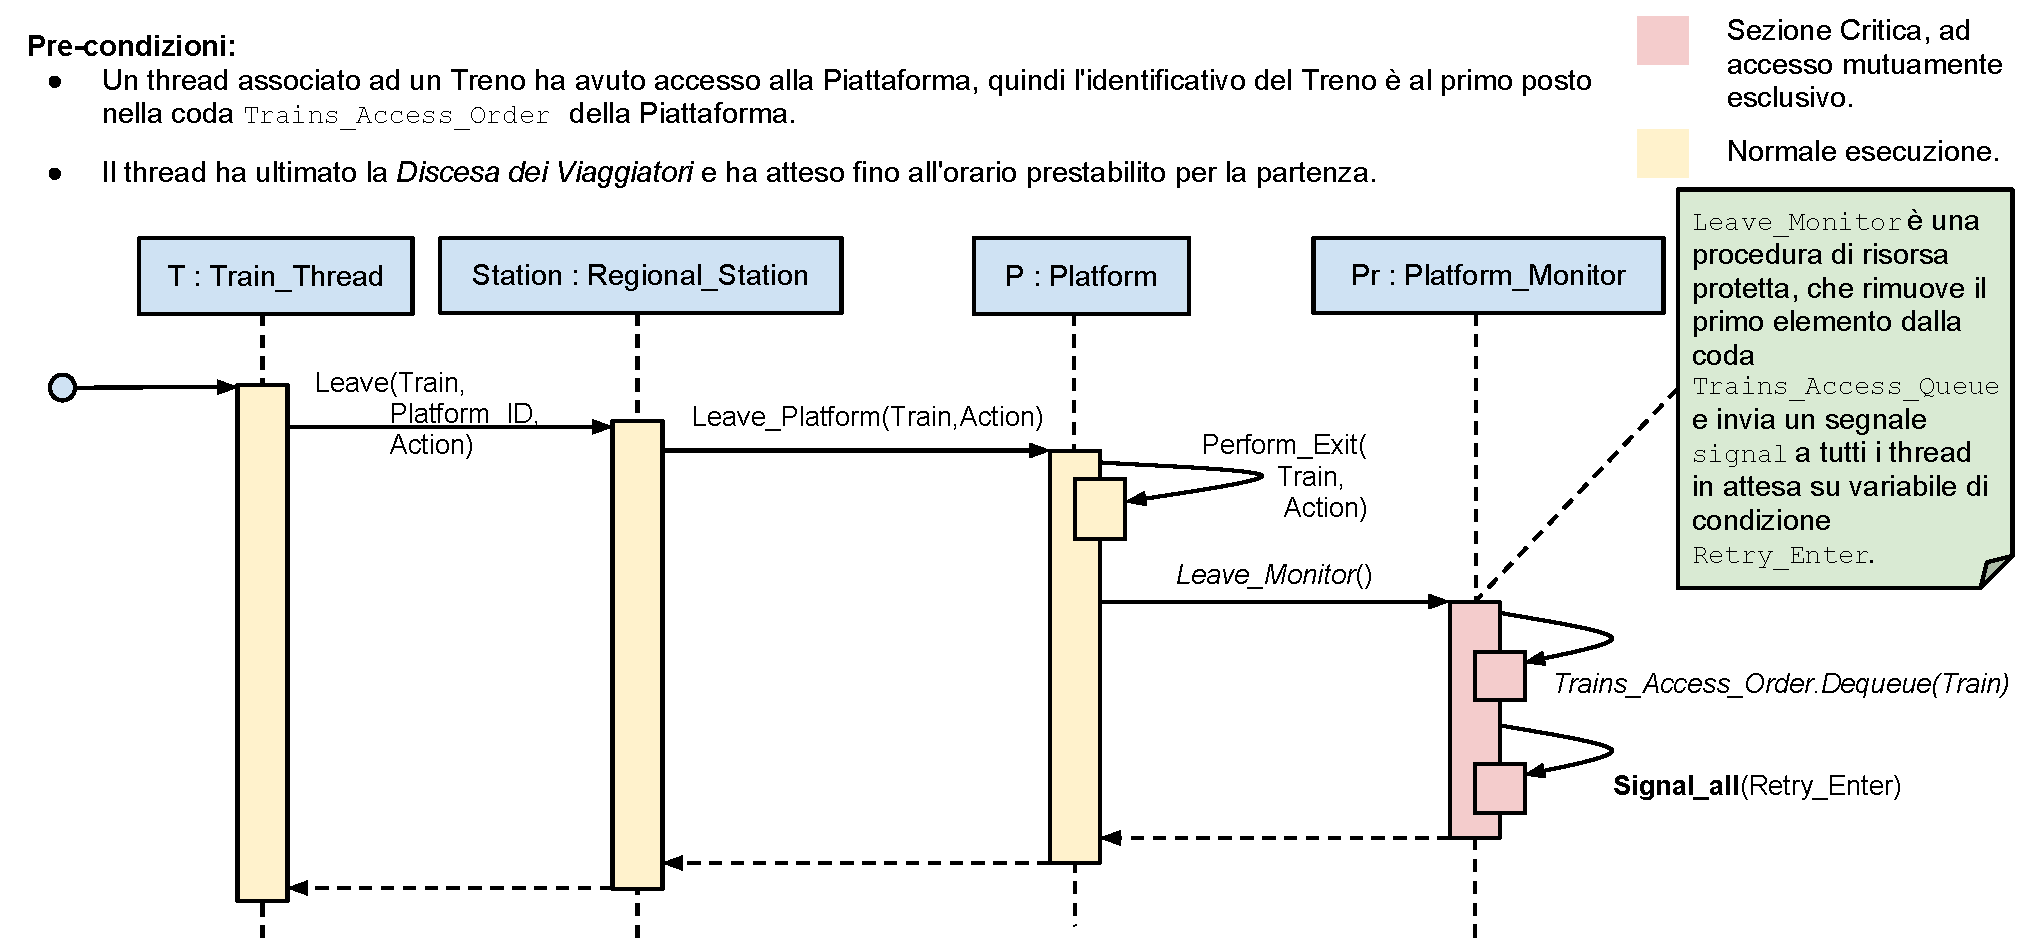
\includegraphics[trim = 30mm 0mm 0mm 0mm,scale=0.5]{imgs/platform_exit_Sequence_Diagram.pdf}
			\caption{\footnotesize{Diagramma di Sequenza, operazioni necessarie per l'uscita da una Piattaforma.}}
			\label{fig:platform_access}
		\end{figure}
		
		L'uscita da una Piattaforma $P$ necessita di due prerequisiti principali:
		
			\begin{itemize}
				\item Il thread che gestisce il Treno ha prima effettuato l'ingresso, e quindi \ttt{Free = False} presso la risorsa a protezione della Piattaforma, ed è già stata effettuata la Discesa dei Passeggeri (se prevista dal Percorso del Treno).
				\item \'E stato generato l'evento che notifica l'arrivo dell'orario previsto per la partenza.
			\end{itemize}
		
		A questo punto, le operazioni effettuate (eseguite in mutua esclusione dal thread corrente) sono:
		
			\begin{itemize}
				\item Viene effettuata la Salita dei Viaggiatori in attesa presso $P$.
				\item La risorsa viene rilasciata dal Treno in esecuzione, cambiando il valore del flag \ttt{Free} a \ttt{True}.
			\end{itemize}
		
		La \bb{Salita dei Viaggiatori} è simile alla discesa dei Passeggeri presentata al punto precedente. Essa viene eseguita in mutua esclusione, ed è composta dalle seguenti azioni:
		\begin{itemize}
			\item Viene estratto ciascun Viaggiatore $V$ dalla coda \ttt{Leaving\_Queue} di $P$, e per ciascuno di essi:
			\begin{itemize}
				\item Se il Treno atteso da $V$ (informazione recuperabile dalla Tappa corrente del suo Biglietto) è proprio il Treno correntemente in esecuzione $T$ e \ii{se la capienza massima di $T$ non è stata raggiunta} allora:
					\begin{itemize}
						\item il numero di posti occupati di $T$ viene incrementato;
						\item l'Operazione \ttt{ENTER} del Viaggiatore viene inserita:
					\end{itemize}
				\item Se $T$ invece non è il Treno atteso da $V$, quest'ultimo viene reinserito nella coda \ttt{Leaving\_Queue}.
			\end {itemize}
		\end{itemize}
	\end {description}

	Anche in questo caso, le operazioni che attuano la discesa dei passeggeri possono essere eseguite internamente alla sezione critica definita dalla risorsa a protezione della Piattaforma, o esternamente, per poi permettere l'acquisizione da parte di un altro Treno liberandola (\ttt{Free = True}). Anche in questo caso ho preferito la seconda soluzione.

% ############################################################################################################
% ########################################### ACCESSO_STAZIONE_GATEWAY #######################################
% ############################################################################################################		

	\subsubsection{Accesso ad una Stazione di Gateway}\label{subsubsec:gateway_stations_func}
	
	Alcuni Treni seguono percorsi che attraversano più Regioni. Tra le tappe che compongono tali percorsi, alcune indicheranno l'attraversamento di Regioni di Gateway, introdotte nella sezione \ref{sec:gateway_stations}. 
	Le azioni di Ingresso, Salita dei Viaggiatori, e Ripartenza presso questo tipo di stazioni seguono le stesse regole descritte per le stazioni Regionali nella sezione \ref{subsubsec:regional_station_access}. Esse hanno quindi un effetto locale alle Regioni (nodi) di provenienza e di destinazione.
	Per quanto riguarda invece la Discesa dei Viaggiatori, essa può prevedere un \ii{trasferimento remoto} dei Viaggiatori in attesa di arrivo.
	
	Il Passaggio di un Treno da una regione alla successiva può essere schematizzato come segue: siano $G1$ e $G2$  Stazioni di Gateway connesse, che collegano le regioni $R1$ ed $R2$, con $G1 \in R1$, e sia $G2 \in R2$. Un Percorso che attraversa i due Gateway conterrà almeno una Tappa $T1$ tale per cui il campo \ttt{next\_station} avrà il valore $G1$, \ttt{destination\_platform} una delle Piattaforme possibili per effettuare l'accesso $P$, e \ttt{region} la regione $R1$, e una tappa $T2$ tale per cui il campo \ttt{next\_station} avrà il valore $G2$, \ttt{destination\_platform} la stessa piattaforma specificata in $T$, e \ttt{region} la regione $R2$.
	Le operazioni eseguite saranno le seguenti:
	\begin{itemize}
		\item Il Treno corrente $T$ effettua l'accesso alla Stazione $G1$, Piattaforma $P$.
		
		\item $T$, se previsto dal Percorso, effettua Discesa dei Viaggiatori. Tale azione è simile alla Discesa descritta in sezione \ref{subsubsec:regional_station_access}, ma se un Viaggiatore una volta sceso proseguirà il proprio percorso su un nodo diverso da quello corrente, esso verrà trasferito mediante messaggio remoto al nodo successivo, e solo a questo punto verrà inserita l'Operazione \ttt{ENTER} del Viaggiatore nella coda di operazioni di \ttt{Traveler\_Pool} locale al nodo destinazione.
		
		\item Il descrittore del Treno corrente $D_T$ viene serializzato (\ii{marshalling}), e inviato tramite invocazione remota alla Stazione di Gateway della Regione $G2$ ad essa connessa. L'individuazione dell'indirizzo della regione specificata nel parametro \ttt{region}, avviene interrogando il \ttt{Name\_Server}, se esso non è già presente in una cache locale.
		\item Il flusso ciclico di istruzioni eseguite dal thread che gestisce $T$ viene interrotto (esso potrà così ottenere un nuovo Descrittore di Treno ed eseguire per esso le proprie operazioni).
		\item Presso la regione $R2$, stazione di Gateway $G2$, vengono eseguite le seguenti operazioni:
			\begin{itemize}
				\item Il Descrittore viene de-serializzato (\ii{unmarshalling}).
				\item I dati del Descrittore $D_{T'}$ presenti nella regione $R2$ vengono aggiornati con quelli ricevuti.
				\item Viene ottenuta la Piattaforma in mutua esclusione e ne viene impostato il campo \ttt{Free} a \ttt{False}.
				\item Vengono operate attesa fino all'orario di partenza previsto (secondo il clock del nodo corrente), Salita dei Viaggiatori e Partenza dalla Stazione come per le Stazioni Regionali.
				\item Viene restituito un messaggio di \ii{acknowledgement} al nodo $R1$, che comunica l'avvenuta esecuzione delle operazioni.
			\end{itemize}
		\item Una volta ricevuto il messaggio di \ii{acknowledgement}, presso il nodo $R1$, viene liberata la piattaforma corrente (\ttt{Free} viene impostato a \ttt{True}) in modo tale da permettere ad altri Treni di occuparla.
	\end{itemize}
	
	Ciò che garantisce la correttezza della soluzione presentata, relativamente a discesa e salita dei passeggeri locale, è la modalità con la quale il Viaggiatore viene accodato presso la Stazione di Gateway come descritto nella sezione \ref{subsec:percorrenza_viaggiatore}, ovvero in modo tale per cui:
	\begin{itemize}
		\item Presso le coda \ttt{Arrival\_Queue} delle Piattaforme nel nodo di partenza vi saranno tutti e soli i passeggeri in attesa di scendere presso la Stazione di Gateway, se previsto dal loro Biglietto.
		\item Presso le code \ttt{Leaving\_Queue} delle Piattaforme nel nodo di destinazione vi saranno invece solamente i Viaggiatori che vogliono raggiungere una destinazione interna al nodo corrente.
	\end{itemize}  
	Si noti che la soluzione riportata prevede lo scambio di due messaggi remoti, il primo per la transizione del Treni tra le Regioni, e il secondo di acknowledgement per poter liberare la risorsa Piattaforma presso il nodo di partenza. Di fatto, data l'inaffidabilità della rete, è possibile che uno dei due messaggi scambiati non venga ricevuto dal nodo di destinazione. Abbiamo quindi due casi:
		\begin{itemize}
			\item \ii{L'invio del primo messaggio fallisce.} In questo caso, il flusso di esecuzione del thread che gestisce il Treno viene interrotto. Per semplicità si può pensare che il Treno sia cancellato a causa di un guasto, o si può ridurre il Percorso fino alla Tappa che ha causato l'errore, dopo essersi accertati dell'effettiva irraggiungibilità del nodo destinazione.
			\item \ii{Il messaggio di acknowledgement non viene consegnato.} In questo caso il problema è più grave. Il Treno presso il nodo di destinazione continua la propria corsa, mentre la Piattaforma abbandonata rimane occupata, e quindi inutilizzabile dai Treni che sopraggiungono. Per risolvere questo tipo di problema è possibile prevedere un tempo massimo di occupazione della Piattaforma, oltre il quale richiedere l'effettivo stato di occupazione della Piattaforma presso la Stazione di Gateway della Regione di destinazione e, nel caso in cui risultasse libera, procedere alla liberazione della stessa, impostando \ttt{Free} a \ttt{True}. 
		\end{itemize}
	 
	
